\section{Anexos}
\subsection{Carpeta de laboratorio}
\href{https://drive.google.com/drive/folders/1-pCu1uoGqFwTV82Zj6AoLYSWdHQhPP2F?usp=drive_link}{\textbf{Enlace}} de acceso a la carpeta de Google Drive con simulaciones y evidencias del laboratorio.


\subsection{Stack Pointer}

Incialización del Stack Pointer:

\begin{verbatim}
RESET:
    cli ldi r16, high(RAMEND)
    out SPH, r16
    ldi r16, low(RAMEND)
    out SPL, r16 sei
    ; ...
\end{verbatim}

Usos del Stack Pointer: rcall, call, interrupciones
preservacion de datos entre subrutinas e ISRs

\begin{verbatim}
MI_ISR:
    push r16
    out r16, SREG
    push r16
    ; ... 
    pop r16
    in SREG, r16
    push r16
    reti
\end{verbatim}

\section{Timer 1}

El prescaler del Temporizador 1 es configurado a través del registro TCCR1B el cual posee la siguiente configuración:

\begin{figure}[H]
  \centering
  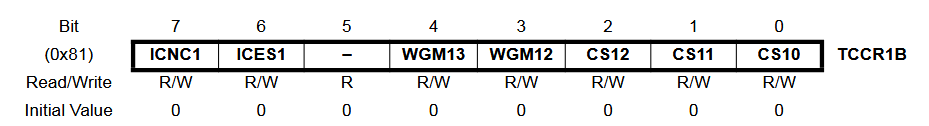
\includegraphics[width=\linewidth]{./Anexos/Marco Teorico/Timers/TCCR1B.png}
  \caption{Registro de control B (TCCR1B) para Timer/Counter1. Fuente: hoja de datos del ATmega328P\@\cite{atmega328p_datasheet}.}
  \label{fig:TCCR1B}
\end{figure}

Los bits CS12 CS11 y CS10 configuran el prescaler del timer conforme a la siguiente tabla: 

\begin{figure}[H]
  \centering
  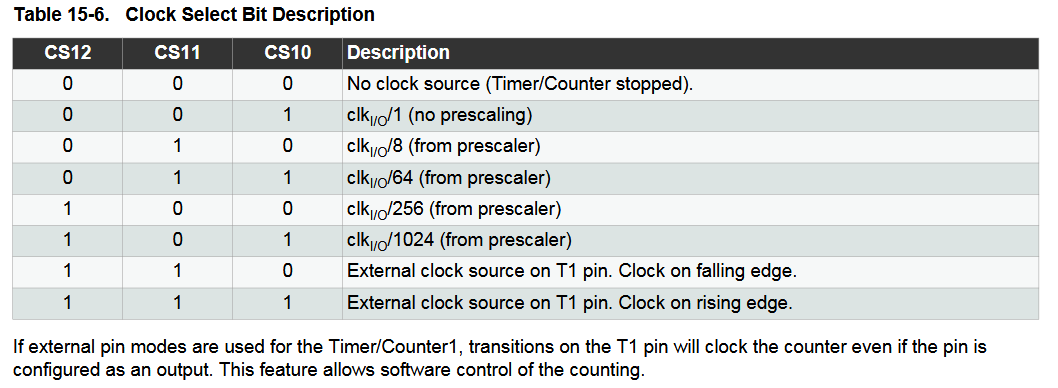
\includegraphics[width=\linewidth]{./Anexos/Marco Teorico/Timers/Prescaler Table.png}
  \caption{Clock Select (CS12:0) opciones de prescaler para Timer/Counter1. Fuente: hoja de datos del ATmega328P\@\cite{atmega328p_datasheet}.}
  \label{fig:prescaler-table}
\end{figure}


El máximo valor de tiempo que admite el Timer 1 (de 16 bits) con el prescaler de 1024 es de 4.19 segundos (aproximadamente). Para valores más grande de delay será necesario crear un contador de overflow aparte utilizando registros de uso general o SRAM

Este es un ejemplo de inicialización de timer 1 para un overflow de 1s

\begin{verbatim}
ldi r16, 0b101       sts TCCR1B, r16
ldi r16, HIGH(49911) sts TCNT1H, r16
ldi r16, LOW(49911)  sts TCNT1L, r16 
\end{verbatim}

El primer registro (TCCR1B) determina el prescaler del reloj (según la figura\ \ref{fig:prescaler-table})

Utilizando la tabla de vectores de interrupcion que se muestra en la figura\ \ref{fig:interrupt-vectors} se mapea el vector de interrupción con la etiqueta del ISR correspondiente:

\begin{verbatim}
.org 0x001A rjmp TIMER1_OVF_ISR

TIMER1_OVF_ISR:
    push r16
    out r16, SREG
    push r16
    ; ... 
    pop r16
    in SREG, r16
    push r16
    reti
\end{verbatim}

\subsection{Interrupciones Externas}
   \subsubsection{EINT}
    Interrupciones externas 

    \begin{figure}[H]
    \centering
    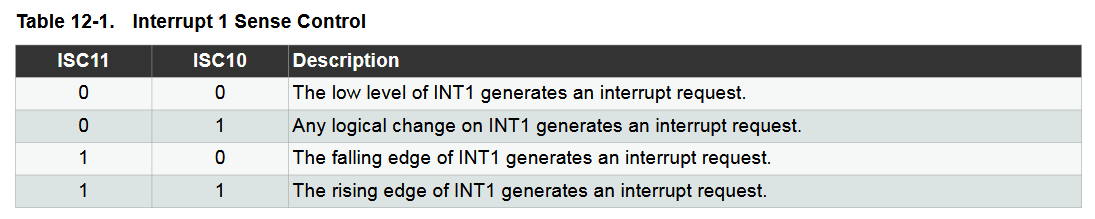
\includegraphics[width=\linewidth]{./Anexos/Marco Teorico/External Interrupts/EICRA table.png}
    \caption{Tabla de configuraciones para EICRA. Fuente: hoja de datos del ATmega328P\@\cite{atmega328p_datasheet}.}
    \label{fig:EICRA-table}
    \end{figure}

    \begin{figure}[H]
    \centering
    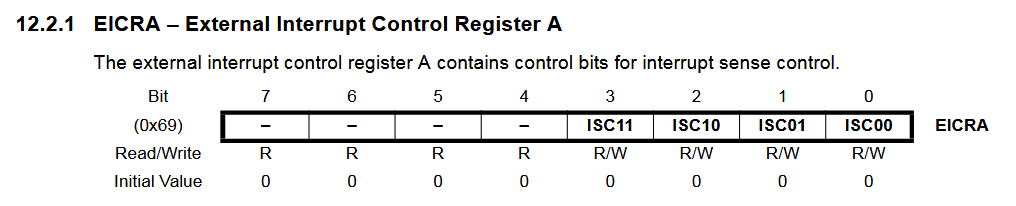
\includegraphics[width=\linewidth]{./Anexos/Marco Teorico/External Interrupts/EICRA.png}
    \caption{Registro de configucación de interrupciones externas EICRA. Fuente: hoja de datos del ATmega328P\@\cite{atmega328p_datasheet}.}
    \label{fig:EICRA}
    \end{figure}

    \begin{figure}[H]
    \centering
    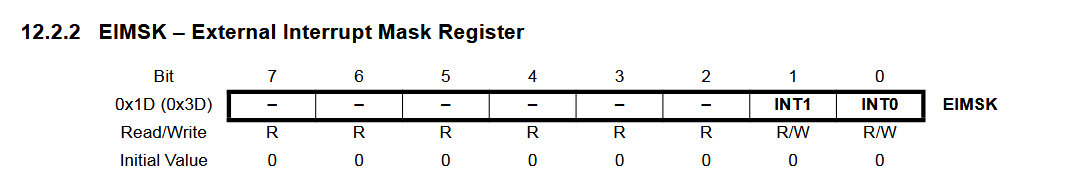
\includegraphics[width=\linewidth]{./Anexos/Marco Teorico/External Interrupts/EIMSK.png}
    \caption{Registro de configucación de máscaras de interrupciones externas EICRA. Fuente: hoja de datos del ATmega328P\@\cite{atmega328p_datasheet}.}
    \label{fig:EIMSK}
    \end{figure}

    \subsubsection{PCINT}
    Interrupciones por cambio en PIN


    \begin{figure}[H]
    \centering
    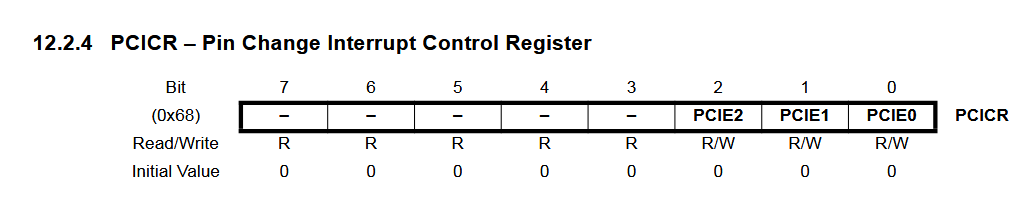
\includegraphics[width=\linewidth]{./Anexos/Marco Teorico/External Interrupts/PCICR.png}
    \caption{Registro de configucación interrupciones PCICR (PCINT). Fuente: hoja de datos del ATmega328P\@\cite{atmega328p_datasheet}.}
    \label{fig:PCICR}
    \end{figure}

    \begin{figure}[H]
    \centering
    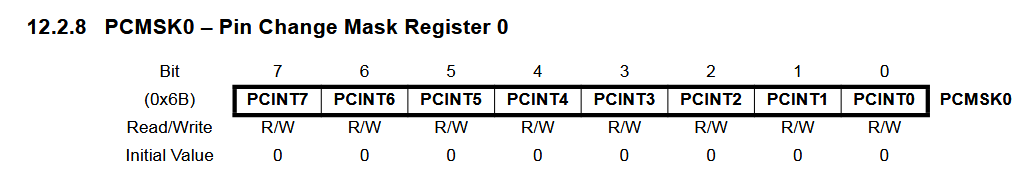
\includegraphics[width=\linewidth]{./Anexos/Marco Teorico/External Interrupts/PCMSK.png}
    \caption{Registro de configucación de mascara de pines para interrupciones PCIMSK0 (PCINT). Fuente: hoja de datos del ATmega328P\@\cite{atmega328p_datasheet}.}
    \label{fig:PCIMSK}
    \end{figure}

\subsection{SRAM}

\begin{verbatim}
.dseg
variable: byte 1  
arreglo: byte 100
\end{verbatim}

% Como leer de sram

\subsection{FLASH}

\begin{verbatim}
.cseg
.org 0x300 TABLA:
    .db 0xFF, 0x30, 0x30, 0xFF
\end{verbatim}

\begin{verbatim}
GET_DATA:
    ldi ZH, high(TABLA<<1)
    ldi ZL, low(TABLA<<1)
    lpm r16, Z+
    ret
\end{verbatim}

% USART

\subsection{USART Asíncrono}
    \subsubsection{Inicialización}
    \begin{verbatim}
    .equ _F_CPU = 16000000
    .equ _BAUD = 9600
    .equ _BPS = (_F_CPU/16/_BAUD) - 1

    .org 0x0024 rjmp USART_RX_ISR
    
    RESET:
    ; Configurar baudios
    sts UBRR0H, high(_BPS)
    sts UBRR0L, low(_BPS)

    ; Habilitar: receptor, transmisor
    ; e interrupciones por RX
    ldi r16, 0b10011000
    sts UCSR0B,r16

    ; Establecer formato:
    ; 8 data bits, 2 stop bits
    ldi r16, (1<<USBS0)|(3<<UCSZ00)
    sts UCSR0C,r16

    sei
    \end{verbatim}
    \subsubsection{Transmisión}
    \begin{verbatim}
    ldi r16, 0x3f ; Cargar r16 
    sts  UDR0, r16 ; Transmitir
    \end{verbatim}
    \subsubsection{Recepción}

    \begin{verbatim}
    USART_RX_ISR:
    push r16 
    in r16, SREG 
    push r16 

    ; Datos recibidos en r16
    lds r16, UDR0
    ; ...

    pop r16
    out SREG, r16
    pop r16	
    reti
    \end{verbatim}
    
\subsection{USART asíncrono con Ring Buffer}

    \subsubsection{Inicialización}
    \begin{verbatim}
    .dseg ; Ring buffer ram alocation
    tx_buffer: .byte TX_BUF_SIZE  
    tx_head:   .byte 1            
    tx_tail:   .byte 1           

    .cseg
    .equ TX_BUF_SIZE = 256
    .equ TX_BUF_MASK = TX_BUF_SIZE - 1

    .equ _F_CPU = 16000000
    .equ _BAUD = 57600 
    .equ _BPS = (_F_CPU/16/_BAUD) - 1
    
    ; Recieved USART data
    .org 0x0024 rjmp USART_RX_ISR	
    ; USART Data register clear
    .org 0x0026 rjmp USART_UDRE_ISR 

    RESET:
    clr r1

    ; Stack 
    ldi r16, high(RAMEND) out SPH, r16
    ldi r16, low(RAMEND)  out SPL, r16

    ; Init USART
    ldi r16, low(_BPS)
    ldi r17, high(_BPS)
    rcall USART_INIT

    sei
    ; ...

    USART_INIT:	
    sts  tx_head, r1
    sts  tx_tail, r1

    sts UBRR0H, r17
    sts UBRR0L, r16

    ldi r16, 0b10011000
    sts UCSR0B,r16

    ldi r16, (1<<USBS0)|(3<<UCSZ00)
    sts UCSR0C,r16
    ret
    \end{verbatim}


    \subsubsection{Subrutina USART WRITE BYTE}
    \begin{verbatim}
    USART_WRITE_BYTE:
    push r17
    push r18
    push r19
    push ZH
    push ZL

    ; head/tail
    lds  r17, tx_head
    lds  r18, tx_tail

    ; r16 -> next = (head + 1) & MASK 
    mov  r19, r17
    inc  r19
    andi r19, TX_BUF_MASK 
    ; Clamping:
    ; Con 256 es 0xFF: no cambia, 
    ; pero deja claro el patrón

    wait_space: 
    ; buffer lleno? next == tail
    lds  r18, tx_tail
    cp   r19, r18
    breq wait_space ; espera activa

    have_space:
    ; Z -> Cabeza de buffer
    ldi  ZL, low(tx_buffer)
    ldi  ZH, high(tx_buffer)
    add  ZL, r17 
    adc  ZH, r1

    st   Z, r16 ; Guardar en buffer

    ; Cabeza = next
    sts  tx_head, r19

    ; Habilitar interrupcion UDRE
    ; así el ISR comienza/continúa 
    ; drenando el buffer
    cli
    lds  r18, UCSR0B
    ori  r18, (1<<UDRIE0)
    sts  UCSR0B, r18
    sei

    pop  ZL
    pop  ZH
    pop  r19
    pop  r18
    pop  r17
    ret
    \end{verbatim}


    \subsubsection{Interrución USART UDRE ISR}
    \begin{verbatim}
    USART_UDRE_ISR:
    push r16
    in   r16, SREG
    push r16
    push r17
    push r18
    push r20
    push ZH
    push ZL

    ; r17 = head, r18 = tail
    lds  r17, tx_head
    lds  r18, tx_tail

    ; buffer vacío? head == tail
    cp   r17, r18
    brne usart_udre_send

    ; vacío: deshabilitar UDRIE0
    lds  r20, UCSR0B
    andi r20, ~(1<<UDRIE0)
    sts  UCSR0B, r20
    rjmp usart_udre_exit

    usart_udre_send:
    ; Z -> Cola de buffer
    ldi  ZL, low(tx_buffer)
    ldi  ZH, high(tx_buffer)
    add  ZL, r18
    adc  ZH, r1 

    ; Transmitir byte
    ld   r16, Z
    sts  UDR0, r16

    ; cola = (cola + 1)
    inc  r18                
    andi r18, TX_BUF_MASK 
    ; Clamping:
    ; Con 256 es 0xFF: no cambia, 
    ; pero deja claro el patrón

    sts  tx_tail, r18

    usart_udre_exit:
    pop  ZL
    pop  ZH
    pop  r20
    pop  r18
    pop  r17
    pop  r16
    out  SREG, r16
    pop  r16
    reti
    \end{verbatim}

    
    \subsubsection{Interrución USART RX ISR}
    \begin{verbatim}
    USART_RX_ISR:
    push r16 
    in r16, SREG
    push r16

    lds r16, UDR0 
    ; ...

    pop r16
    out SREG, r16
    pop r16
    reti
    \end{verbatim}